% -----------------------------------------------------------------
% => Ambiente Interno
% -----------------------------------------------------------------

\subsection{Ambiente Interno de Aprendizagem}
\label{section:wIndoorClassroom}

%Abordagens de construção de ambientes ou componentes de sala de aula presencial tem sido objeto de estudo de alguns trabalhos, em geral, esses trabalhos enfocam o uso de RFID (\textit{Radio-Frequency IDentification}), câmeras, servidores, novos tipos de mobiliário, lousas inteligentes e dispositivos móveis.

\cite{Bargaoui:2014} apresentam um \textit{Gateway} para conectar os múltiplos dispositivos utilizados numa sala de aula inteligente. Para construção da solução são utilizados RFID, servidor de dados, ferramentas de administração, lousa inteligente, \textit{Raspberry-Pi}, OSGi (\textit{Open Service Gateway Initiative}) e dispositivos inteligentes diversos. Como trabalhos futuros, é sugerida a criação de um modelo de avaliação da experiência do estudante e compará-lo com uma sala de aula clássica.

\cite{Margetis:2011} descrevem uma abordagem a partir da aplicação de Inteligência de Ambientes em sala de aula e faz um levantamento de requisitos importantes a serem levados em consideração a fim de ajudar de modo mais eficiente na melhoria da educação dos estudantes. Utiliza um \textit{framework} chamado ClassMATE (\textit{Classroom Multiplatform Augmented Technology Environment}) dentre outras ferramentas como: FAMINE (\textit{FORTH's AMI Network Environment}), PERSONAF (\textit{Personalised Pervasive Scrutable Ontological Framework}), \textit{Learning Technology Systems Architecture} (LTSA), Desk aumentado, lousa inteligente, PUPIL (um \textit{front-end educacional}) que são aplicações eletrônicas para sala de aula (Figura~\ref{fig:margetis2011}).

\begin{figure}[ht]
\centering
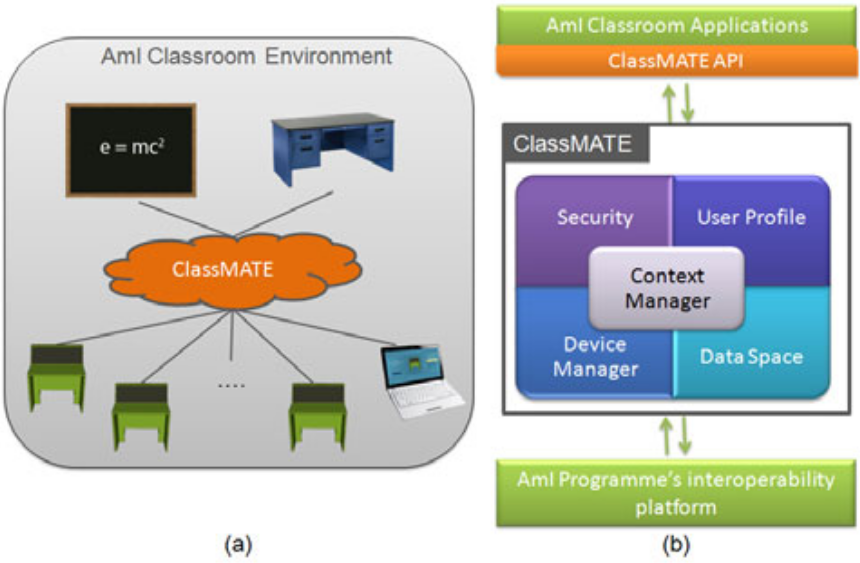
\includegraphics[width=0.8\linewidth]{imgs/margetis2011}
\caption{(a) Cenário do ClassMATE. (b) Arquitetura do ClassMATE}
\label{fig:margetis2011}
\end{figure}

\cite{Chang:2014} apresentam soluções de transformação de salas de aula tradicionais em salas de aula inteligentes baseadas em Internet das Coisas (IoT). Apresentam a definição de uma estrutura IoT composta por quatro camadas: \textit{Perceptive Layer, Network Layer, Processing Layer, Application Layer}. Afirma que há uma relação entre essas camadas e uma sala de aula. Assim, para tornar uma escola tradicional uma escola inteligente é necessário atingir três pontos:

\begin{enumerate}
   \item "Transformar uma sala de aula tradicional em uma IoT-base" através da instalação de um Set-top-box (STB) com webcam, RFID, Wifi e outras ferramentas de transmissão de dados (Figura~\ref{fig:chang2014}).
   \item Analisar o comportamento de aprendizagem dos alunos usando o RFID instalado no STB para identificar individualmente a presença do aluno na sala, além de enviar informações das respostas dos exercícios no \textit{tablet} ou \textit{smartphone} para gerar estatísticas relativas ao desempenho e às dificuldades dos alunos em determinado conteúdo de uma disciplina;
   \item Gerenciar dispositivos inteligentemente usando \textit{tablet} se comunicando através de Zigbee\footnote{Tecnologia de comunicação sem fio desenvolvida pela \textit{Zigbee Alliance} como padrão global aberto visando baixos custo e consumo de energia~\citep{Digi:2017}} para controlar dispositivos como projetor, ventilador, ar-condicionado e luzes.
\end{enumerate}

Ao detalhar os componentes de cada um desses pontos, o artigo apresenta em qual camada IoT um componente específico está localizado.

\begin{figure}[ht]
	\centering
	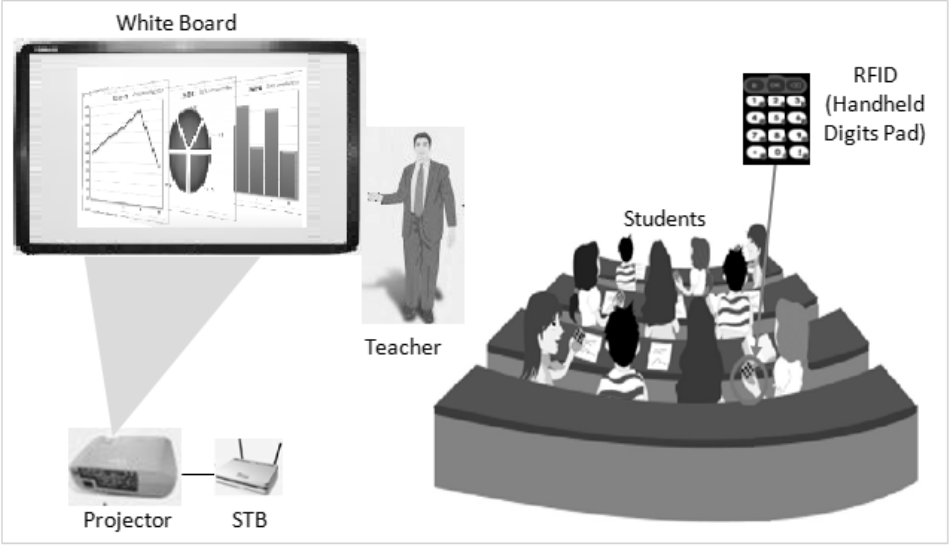
\includegraphics[width=0.8\linewidth]{imgs/Chang2014}
	\caption{Cenário de Sala de Aula Inteligente}
	\label{fig:chang2014}
\end{figure}

\cite{Savvaki:2013} apresentam o projeto de uma nova mesa (desk) para estudantes em uma sala de aula inteligente. A nova configuração utiliza como requisitos de projeto elementos de Estética, Usabilidade, Tecnologia e Viabilidade. Inicialmente, foram projetadas quatro alternativas baseadas no uso de tablet, mas, a versão final propõe um computador \textit{all-in-one} embarcado em uma estrutura que também permite atividades baseadas em papel (Figura~\ref{fig:Savvaki2013}). Duas mesas adjacentes podem se conectar e possibilitar atividades colaborativas e, assim, promover trabalhos em equipe.

\begin{figure}[ht]
\centering
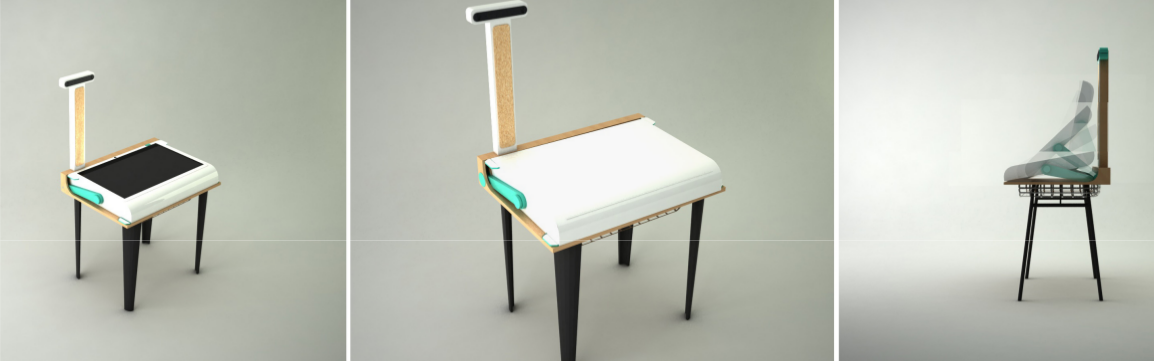
\includegraphics[width=0.9\linewidth]{imgs/Savvaki2013}
\caption{Mesa de estudos inteligente}
\label{fig:Savvaki2013}
\end{figure}

O trabalho de \cite{Zhang:2003} foca em aprendizado remoto que utiliza: protocolo multicast híbrido aplicação-camada, um software dedicado chamado "\textit{SameView}", uma sala de aula inteligente que é uma sala de aula ampliada com telas do tamanho da parede, sensores, câmeras e módulos de percepção e computação associados, alguns tipos de tecnologia de computação de padrões de aprendizagem, aprendizagem de interconexão através de protocolos de comunicação com e sem fio. A ideia é proporcionar maior participação na aula para quem está assistindo remotamente.

\cite{Mathioudakis:2013} apresentam uma abordagem centrada no aluno para dar apoio aos professores na melhoria do processo de aprendizado em ambientes educacionais. O sistema proposto apresenta uma infraestrutura multiagente inteligente que monitora, discretamente, as atividades dos alunos e notifica o professor, em tempo real, sobre as potenciais deficiências e armadilhas que precisam ser tratadas. O trabalho também aborda a questão da identificação do comportamento e análise de estatística de sala de aula.

O trabalho de \cite{Hwang:2009} está contextualizado no ensino da prática de laboratório de Difracção de Raios X de cristal único para pesquisadores inexperientes. O sistema identifica em que parte do laboratório o estudante está e, assim, infere a atividade que será executada por ele. Associando essa informação de contexto à temperatura ambiente, o estudante recebe instruções dos procedimentos que devem ser feitos, por exemplo, a seleção de um cristal de qualidade e tamanho adequado para a atividade a ser feita. Essas instruções são passadas através de um PDA (\textit{Personal Digital Assistant}). A efetividade do sistema foi medida através de pesquisa de opinião com os próprios estudantes que relataram uma melhoria no desempenho e na praticidade das aulas de laboratório.

Para \cite{Santana:2013}, simplesmente utilizar dispositivos móveis em sala de aula não é suficiente, é necessário que esses dispositivos se comuniquem entre si e contribuam com a melhoria do processo de ensino-aprendizagem. Este trabalho descreve a aplicação do conceito de Inteligência de Ambientes para criação de um ambiente educacional adaptado e personalizado, no caso, em escolas mexicanas. Foram utilizadas duas placas (mestre e escrava). A placa mestre (com um microcontrolador Pic18f4550) é a responsável pela interação com a sala de aula inteligente, monitoramento de temperatura, quantidade de luz ambiente, presença do professor para ligar o projetor e um \textit{display LCD} para monitoramento de todos os componentes. Entretanto, nada é explicitamente dito sobre o funcionamento da placa escrava.

\cite{Dekdouk:2012} introduz um ambiente de sala de aula inteligente baseado em "\textit{mobile learning}"~com uso de \textit{tablets}, \textit{RFID} e servidor de gerenciamento do ambiente (\textit{WebCT/Moodle}) focado na interação do estudante com o conteúdo (exemplo de aula de física) através do tablet e de uma lousa inteligente (Figura~\ref{fig:Dekdouk2012}). Nesse ambiente, também é possível fazer trabalhos em grupos. O trabalho apresenta um cenário e um esboço de um protocolo de comunicação, entretanto, não são executados testes e não é feito reconhecimento de atividades ou comportamentos.

\begin{figure}[ht]
	\centering
	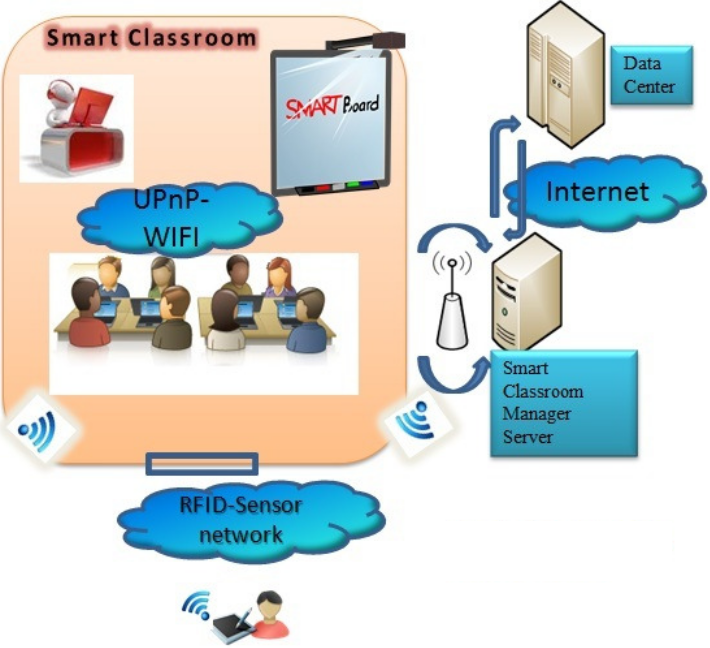
\includegraphics[width=0.6\linewidth]{imgs/Dekdouk2012}
	\caption{Sala de aula inteligente}
	\label{fig:Dekdouk2012}
\end{figure}

\cite{Gligoric:2012} apresentam um sistema de inferência da qualidade de uma palestra com ênfase na aplicação de Internet das Coisas (IoT) em Sala de Aula Inteligente. Neste trabalho é discutido como Inteligência de Ambientes pode ser usada para oferecer um \textit{feedback} automático e em tempo real da qualidade de uma palestra em auditório baseando-se em parâmetros. Utilizando sensores de ruído, \textit{Passive Infrared} (PIR), câmeras de vídeo e microfones. A inferência da qualidade da palestra é feita a partir do nível de interesse da plateia, que pode ser medido pela inquietação dos ouvintes e pelo ruído ambiente. 
